\documentclass[11pt,twoside,a4paper,final]{llncs}
\usepackage[utf8]{inputenc}
\usepackage[T1]{fontenc}
\usepackage[MeX]{polski}
\usepackage{graphicx}
\usepackage{url}
\usepackage{hyperref}
\usepackage{eurosym}
\usepackage{listings}
\bibliographystyle{splncs}

\begin{document}

\date{28 lipca 2013}
\title{Wstępny projekt}

\author{Łukasz Szewczyk}
\institute{Politechnika Warszawska, Wydział Elektroniki i Technik Informacyjnych}
\maketitle


\section{Wstęp}
W tym dokumencie opisuję rozwiązania części z~wymagań stawianych mojej bibliotece.

\section{2.1 Uniwersalny silnik}
\subsection{Podział na warstwy}
Zdecydowałem się podzielić wykres na pięć warstw. Odrysowywanie wykresu będzie się składało z~odrysowania zawartości każdej z~warstw, począwsze od tła, a~na pierwszym planie skończywszy.
Układ warstw został przedstawiony na rysunku~\ref{rys:warstwy}.

\begin{figure}
\centering
\caption{Warstwy wykresu}\label{rys:warstwy}
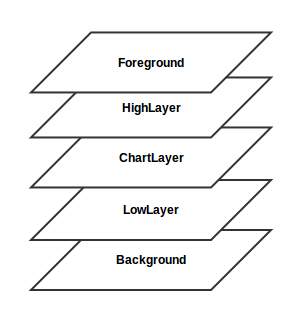
\includegraphics[scale=0.6]{warstwy.png}
\end{figure}

Warstwy tła oraz pierwszego planu służą jedynie odrysowywaniu wzorów przekazanych za pomocą pędzla. Pozostałe warstwy są bardziej złożone i~zawierają liczne elementy.

Warstwy niska i~wysoka są odrysowywane zgodnie z~algorytmem malarza. Służą dodawaniu przez programistów własnych elementów do wykresów istniejących klas.

Warstwa wykresu służy odrysowaniu głównej zawartości wykresu. Tym etapem steruje strategia danego wykresu. W~ogólnym przypadku programiści nie powinni dodawać własnych elementów do tej warstwy.


\section{2.3.1 Wyeksponowanie klas C++ w QML}
\subsection{Adaptery}
Chcąc uniknąć przesadnego rozbudowania interfejsów klas przy jednoczesnym zapewnieniu wysokiego poziomu ich parametryzowalności, podjąłem decyzję o~stworzeniu adapterów dla następujących klas:
\begin{itemize}  
\item{QBrush,}
\item{QPen,}
\item{QFont.}
\end{itemize}
Adaptery te będą dziedziczyć po \textit{QObject}, dzięki czemu staną się możliwe do wyeksportowania do QML. 

\subsection{Eksport do QML}
Klasy wszystkich wysokopoziomowych elementów powinny być pochodnymi klasy QObject. Wszelkie ich parametry, które powinny być konfigurowane przez programistów należy włączyć do zbioru właściwości tej klasy. W~szczególności należy zadbać o~to, aby przy zmianie wartości danej właściwości, i~tylko wtedy, emitować sygnał informujący o~tym zdarzeniu. Jest to niezbędne do poprawnego działania mechanizmu wiązania w~QML. Ponadto, wszystkie metody, które powinny być dostępne z~QML, a~nie są slotami, powinny zostać opatrzone makrem \textit{Q\_INVOKABLE}.

Większość klas powinna być gotowa do wyeksportowania ich do QML za pomocą standardowej procedury, np. poprzez wywołanie funkcji szablonowej
\begin{lstlisting}
template<typename T>
int qmlRegisterType(const char *uri, int versionMajor, 
		    int versionMinor, const char *qmlName)
\end{lstlisting}
Parametrem szablonu jest eksportowany typ, a~parametry funkcji to nazwa modułu, dwie liczby odpowiadające za wersję modułu oraz nazwa pod jaką będzie dostępna eksportowana klasa z~poziomu QML. Qt udostępnia jeszcze kilka innych, specjalizowanych szablonów, np. dla singletonów.\newline

Pozostałe klasy, do wykorzystania ich w~QML, będą wymagały specjalnych interfejsów. Dla klas związanych z~GUI, bazujących na QPainter będzie to QQuickPaintedItem, a~dla tych wykorzystujących SceneGraph -- QQuickItem.


\section{7.2 Wymienność biblioteki}
\subsection{Wersje Qt}
Mogłoby się wydawać, że każde nowe wydanie Qt powinno wymagać ponownej kompilacji projektów zeń korzystających. Tak jednak nie jest. Twórcy Qt zadbali o~to, aby zawsze wtedy kiedy to możliwe, zachowywana była kompatybilność binarna. Oznacza to, że jeśli przy poprawkach do nowej wersji nie zostały zmienione nagłówki klas, a~jedynie ich implementacje, to przebudowanie całej aplikacji nie jest konieczne. Teoretycznie przejście z~Qt~w~wersji 4.8.3 na wersję 4.8.4 może odbyć się jedynie poprzez podmianę plików .dll.

\subsection{QObject}
Klasa QObject jest, jak pisze Scott Meyers w~swojej książce~\cite{meyers}, uchwytem lub kopertą, zawierającą wskaźnik do faktycznej implementacji. Z~kolei klasa implementacji jest nazywana odpowiednio ciałem bądź listem. Taki podział zmniejsza zależności pomiędzy plikami i~znacząco skraca czas kompilacji po zmianach w~kodzie.
Niekiedy ciało ma potrzebę odwołania się do swego uchwytu, np. w~celu wyemitowania sygnału, dlatego musi posiadać do niego wskaźnik. W~Qt przyjęto następującą koncepcję nazewniczą:
\begin{itemize}
\item{uchwyt ma standardową nazwę, zgodną ze swoim przeznaczeniem,}
\item{ciało ma nazwę składającą się z~nazwy swojego uchwytu oraz sufiksu ,,Private''.}
\end{itemize}

\subsection{Optymalizacja}
Można by poprzestać na poprzednim punkcie, jednak twórcy Qt zauważyli możliwość udoskonalenia opisanego tam rozwiązania.
Problem jaki postanowiono rozwiązać dotyczył wielopoziomowych hierarchii dziedziczenia. 
Dla każdego poziomu należy przechowywać po dwa wskaźniki -- uchwyt przechowuje wskaźnik do ciała, a~ciało do uchwytu. Jest to jednak niewielki koszt w~porównaniu do każdorazowej alokacji pamięci dla ciał.
Rozwiązanie tego problemu polega na ograniczeniu liczby powiązań pomiędzy uchwytami i~ciałami. Klasy ciał zostały ułożone w hierarchię dziedziczenia, a~wskaźniki do uchwytu oraz ciała przechowują jedynie klasy najwyższego poziomu. Dodatkowo QObject posiada konstruktor przyjmujący jako argument wskaźnik do ciała, dzięki czemu można je zaalokować tylko raz, w~klasie najniższego poziomu hierarchii dziedziczenia, a~następnie przekazać jako argument konstruktora klasy bazowej. 


Koncepcję podziału na uchwyt oraz ciało zobrazowałem w~kontekście mojej biblioteki na rys.~\ref{rys:dpointer}.
\begin{figure}
\centering
\caption{Przykładowa hierarchia klas}\label{rys:dpointer}
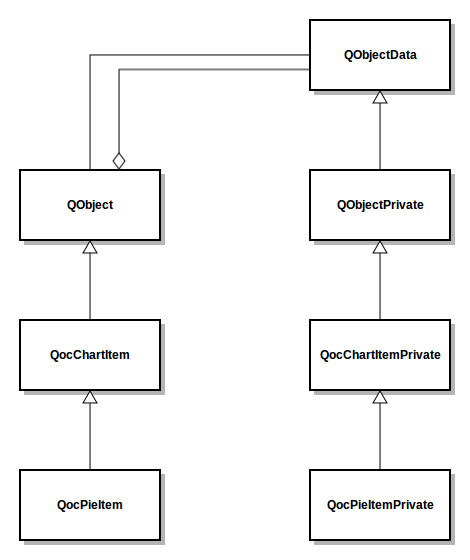
\includegraphics[scale=0.6]{dpointer.png}
\end{figure}

\subsection{Dostęp do uchwytów i ciał}
Optymalizacja opisana w~poprzednim punkcie skutkuje jednak powstaniem pewnego efektu ubocznego.
Wskaźniki do uchwytu i~ciała mają teraz typy klas znajdujących się na szczycie hierarchii dziedziczenia. Dostęp do metod klas pochodnych wymaga rzutowania w~dół. 
Problem ten rozwiązano za pomocą czterech makrodefinicji przyjmujących jako argument nazwę klasy uchwytu. Dwie z~nich należy wywołać w~odpowiednich nagłówkach. Z~kolei pozostałe dwa należy wywoływać na początku każdej metody wymagającej odwołania do ciała lub uchwytu. Miejsce wykorzystania konkretnych makr podaję w~tabelce~\ref{tab:makra}.

\begin{table}[h]\footnotesize
\centering
\caption{Makrodefinicje}
\label{tab:makra}
\begin{tabular}{|c|c|c|}
\hline
Miejsce & Uchwyt & Ciało\\
\hline
Nagłówek & Q\_DECLARE\_PRIVATE & Q\_DECLARE\_PUBLIC\\
\hline
Metoda & Q\_D & Q\_Q\\
\hline
\end{tabular}
\end{table}

\begin{thebibliography}{}
\bibitem[1]{meyers}
,,50 efektywnych sposobów na udoskonalenie Twoich programów'', Scott Meyers, strona 154, 2004, wydawnictwo Helion, ISBN: 83-7361-345-5


\end{thebibliography}
\end{document}
